\section{Theorie}
\label{sec:Theorie}

\subsection{Grundlagen des Ultraschalls}

Als Ultraschall wird eine Welle der Form
\begin{equation}
  p(x,t) = p_0 + v_0 Z \cos{(\omega t - k w)}
\end{equation}
mit Frequenzen im Bereich von $\SI{16}{\kilo\hertz}$ bis $\SI{20}{\kilo\hertz}$ bezeichnet.
Der Faktor
\begin{equation}
  Z = c \rho
\end{equation}
wird als akustische Impedanz bezeichnet, wobei $\rho$ die Dichte des Ausbreitungsmediums bezeichnet und $c$ die Phasengeschwindigkeit im Medium, welche sich für einen Festkörper zu
\begin{equation}
  c_\text{s} = \sqrt{\frac{E}{\rho}}
\end{equation}
sowie für eine Flüssigkeit zu
\begin{equation}
  c_\text{l} = \sqrt{\frac{1}{\kappa \rho}}
\end{equation}
berechnet.
Hierbei steht $E$ für das Elastizitätsmodul und $\kappa$ für die Kompressibilität.\\
Zu Beachten ist außerdem die Ausbreitungsrichtung der Welle, welche in einer Flüssigkeit stets longitudinal ist, in Festkörpern jedoch zusätzlich transversal mit einer Richtungsabhängigen Phasengeschwindigkeit sein kann.
Bei der Ausbreitung kommt es zu einer stark Mediumsabhängigen Abnahme der Intensität der exponentiellen Form
\begin{equation}
  I(x) = I_0 \exp{\alpha x}.
\end{equation}
Die Brechung und Reflexion, welche analog zu elektromagnetischen Wellen stattfindet, wird durch die akustische Impedanz $Z$ in den beteiligten Medien durch den Zusammenhang
\begin{equation}
  R = \bigl( \frac{Z_1 - Z_2}{Z_1 + Z_2} \bigr)^2
\end{equation}
für den Reflexionskoeffizient $R$ und den daraus folgenden Transmissionskoeffizient $T = 1-R$ beschrieben.

\subsection{Erzeugung von Ultraschall}
Zur Erzeugung von Ultraschall bietet sich die Nutzung des Piezoeffekts an, bei dem durch elastische Verformung eines Festkörpers eine elektrische Spannung auftritt.
Direkt kann dieser Effekt zum Empfangen von Ultraschallwellen genutzt werden, zur Erzeugung wird der inverse Piezoeffekt genutzt.
Hierbei wird ein Kristall mithilfe eines periodischen elektrischen Feldes in Schwingungen versetzt, so dass Ultraschallwellen entstehen.
Aufgrund ihrer natürlichen physikalischen Eigenschaften bieten sich Quarze gut als Piezokristalle an.

\subsection{Methoden zur Untersuchung mit Ultraschall}
Zur Untersuchung von Proben, beispielsweise in der Medizin, werden grundsätzlich zwei verschiedene Methoden verwendet.
Das Durchschallungsverfahren \ref{fig:dv} arbeitet mit zwei Messsonden, von denen eine als Sender und die andere als Empfänger von Ultraschall dient.
Falls zwischen beiden Sonden eine Fehlstelle vorhanden ist, kann dies an der absinkenden Intensität erkannt werden.\\
Das Impuls-Echo-Verfahren \ref{fig:ie} hingegen arbeitet nur mit einer Sonde, welche gleichzeitig den Ultraschall sendet und empfängt.
Nach der Reflexion eines gesendeten Impulses trifft der Ultraschall wieder auf die Sonde, aus der Laufzeitdifferenz zwischen Senden und Empfangen kann bei bekannter Phasengeschwindigkeit somit aus dem Weg-Zeit-Gesetz auf die Tiefe einer Fehlstelle geschlossen werden.\\
Bei letzerer Variante ist neben der Verwendung von nur einer Sonde somit der Vorteil, dass neben der Existenz der Fehlstelle auch die genaue Tiefe ermittelt werden kann.



 \begin{figure}
     \centering
     \begin{subfigure}{0.48\textwidth}
         \centering
         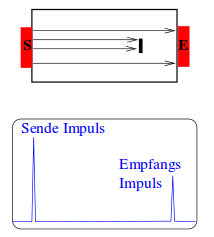
\includegraphics[height=4.5cm]{ressources/dv.png}
         \caption[]%
         {{\small Durchschallungsverfahren.}}
         \label{fig:dv}
     \end{subfigure}
     %\hfill
     \begin{subfigure}{0.48\textwidth}
         \centering
         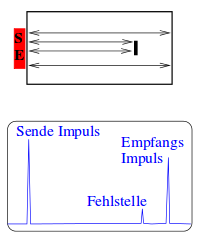
\includegraphics[height=4.5cm]{ressources/ei.png}
         \caption[]%
         {{\small Impuls-Echo-Verfahren.}}
         \label{fig:ie}
     \end{subfigure}
     \caption[]
     {Methoden zur Untersuchung mit Ultraschall. \cite{sample}}
  \end{figure}
%     \vskip\baselineskip
%     \begin{subfigure}[b]{0.475\textwidth}
%         \centering
%         \includegraphics[width=\textwidth]{Abbildungen/Schaltung4.pdf}    % Zahlen vertauscht ... -.-
%         \caption[]%
%         {{\small Schaltung 3.}}
%         \label{fig:Schaltung3}
%     \end{subfigure}
%     \quad
%     \begin{subfigure}[b]{0.475\textwidth}
%         \centering
%         \includegraphics[width=\textwidth]{Abbildungen/Schaltung3.pdf}
%         \caption[]%
%         {{\small Schaltung 4.}}
%         \label{fig:Schaltung4}
%     \end{subfigure}
%     \caption[]
%     {Ersatzschaltbilder der verschiedenen Teilaufgaben.}
%     \label{fig:Schaltungen}
% \end{figure*}
